% 1108.tex
% 研究型文章学习笔记模板
% 建议使用 XeLaTeX 编译(支持中文)
\documentclass[11pt,a4paper]{article}
\usepackage[margin=2.5cm]{geometry}
\usepackage{fontspec}
\usepackage{xeCJK}
\usepackage{amsmath,amssymb}
\usepackage{graphicx}
\usepackage{float}
\usepackage{caption}
\usepackage{booktabs}
\usepackage{enumitem}
\usepackage[colorlinks=true,linkcolor=blue,citecolor=blue,urlcolor=blue]{hyperref}
\usepackage{fancyhdr}
\usepackage{tcolorbox}
\usepackage{datetime}

% 字体(可按需修改)
\setmainfont{TeX Gyre Termes}
\setCJKmainfont{SimSun} % Windows 常见中文字体,视系统调整

% 页眉页脚
\pagestyle{fancy}
\fancyhf{}
% \lhead{\small 研究笔记}
\rhead{\small \PaperMeta}
\cfoot{\small \thepage}

% 元数据命令(在文档开始处填写)
\newcommand{\PaperMeta}{}
\newcommand{\PaperTitle}{}
\newcommand{\PaperAuthors}{}
\newcommand{\PaperVenue}{}
\newcommand{\PaperYear}{}
\newcommand{\PaperLink}{}

% 强调框
\newtcolorbox{highlight}{colback=yellow!10,colframe=yellow!60!black,boxrule=0.5pt}

\begin{document}

% ————— 填写元数据 —————
\renewcommand{\PaperTitle}{Observation and Modulation of the Quantum Mpemba Effect on a Superconducting Quantum Processor}
\renewcommand{\PaperAuthors}{Yueshan Xu, Cai-Ping Fang, Bing-Jie Chen, Ming-Chuan Wang}
\renewcommand{\PaperVenue}{ArXiv}
\renewcommand{\PaperYear}{2025}
\renewcommand{\PaperLink}{http://arxiv.org/abs/2508.07707}
\renewcommand{\PaperMeta}{\PaperTitle\ --- \PaperYear}

% ————— 路径设置 —————
\newcommand{\paperpath}{D:/B_Dr/arXiv-2508.07707v1/}
\graphicspath{{\paperpath}}

\begin{center}
    {\LARGE \textcolor{blue}{\PaperTitle}}\\[6pt]
    {\small \PaperAuthors \quad | \quad \PaperVenue \quad | \quad \PaperYear}\\
    {\small \url{\PaperLink}}
\end{center}

\tableofcontents
\vspace{6pt}
\hrule
\vspace{10pt}

% ————— 快速摘要 —————
\section*{快速摘要(TL;DR)}
\begin{enumerate}[leftmargin=*]
    \item 3--5 行总结核心思想、主要贡献、适用场景与效果。
    \item 一句话亮点:例如“提出了一个轻量级的...,在 X 数据集上将误差降低了 Y\%”。
\end{enumerate}

\section{背景介绍}
\begin{enumerate}[leftmargin=*]
    \item In non-equilibrium quantum many-body systems, the quantum Mpemba effect (QME) emerges as a counterintuitive phenomenon: systems exhibiting greater initial symmetry breaking restore symmetry faster than those with less.
    \item \textcolor{blue}{Three major research fields}
        \begin{itemize}
        \item The Mpemba effect, originally observed as faster freezing of hotter water than colder water under identical conditions, represents a counterintuitive non-equilibrium phenomenon with debated mechanisms.
        \item In open quantum systems interacting with an external environment through Markovian and non-Markovian processes. It is dominated by classical fluctuations, resembling the classical Mpemba effect
        \item In isolated quantum systems governed by intrinsic quantum dynamics. It is driven by intrinsic quantum fluctuations. \textcolor{blue}{In isolated quantum systems, the quantum Mpemba effect (QME) manifests as a remarkable phenomenon: subsystems with greater initial symmetry breaking restore symmetry faster under a symmetry-preserving Hamiltonian.} The type of system under the study:
        \begin{itemize}
            \item Quasiparticle framework for integrable systems that include 1D or 2D models.
            \item In chaotic systems using random and dualunitary circuits.
            \item Non-ergodic contexts, such as many-body localized (MBL) systems
            \end{itemize}
        \end{itemize}
    \item 伪代码/核心算法要点
\end{enumerate}


\section{实验方案}
\begin{enumerate}
    \item Here, we report the observation and control of QME using a superconducting processor featuring a unique fully connected, tunable-coupling architecture that enables precise modulation from short- to long-range interactions.
    \item 调控参量
        \begin{enumerate}
            \item interaction range
            \item potential engineering 
            \item initial state selection
        \end{enumerate}
\end{enumerate}

\subsection{哈密顿量}


实验系统由 16 个超导量子比特组成,采用全连接环状拓扑结构,具备可调耦合能力。系统的有效哈密顿量可写为:

\begin{equation}
H = \sum_{i < j} g_{ij} (\sigma^{+}_{i} \sigma^{-}_{j} + \sigma^{-}_{i} \sigma^{+}_{j}) + \sum_{i} h_i \sigma^{+}_{i} \sigma^{-}_{i}
\end{equation}

其中:
\begin{itemize}
    \item $g_{ij}/2\pi$ 表示量子比特 $Q_i$ 与 $Q_j$ 之间的耦合强度;
    \item $\sigma^{+}_{i}$ 和 $\sigma^{-}_{i}$ 分别为第 $i$ 个量子比特的升降算符;
    \item $h_i/2\pi$ 表示通过频率调制实现的在位势能,参考频率为 $\omega_{\text{ref}}/2\pi \approx 4.24\ \text{GHz}$。
\end{itemize}

为了区分不同耦合范围,我们将耦合强度分为两部分:
\begin{equation}
\begin{aligned}
H &= \sum_{i, j=i+1} g_N (\sigma^{+}_{i} \sigma^{-}_{j} + \sigma^{-}_{i} \sigma^{+}_{j}) \\
&\quad + \sum_{i < j, j \neq i+1} g_L (\sigma^{+}_{i} \sigma^{-}_{j} + \sigma^{-}_{i} \sigma^{+}_{j}) + \sum_{i} h_i \sigma^{+}_{i} \sigma^{-}_{i}
\end{aligned}
\end{equation}

其中:
\begin{itemize}
    \item $g_N/2\pi$ 表示最近邻(短程)耦合强度;
    \item $g_L/2\pi$ 表示长程耦合强度。
\end{itemize}

定义耦合比 $r = |g_N / g_L|$,用于量化不同相互作用区间:
\begin{itemize}
    \item $r \gg 1$:强短程耦合区间;
    \item $r \approx 1$:中间耦合区间;
    \item $r \ll 1$:弱短程耦合区间。
\end{itemize}

通过调节中心总线谐振器频率 $\Delta_{RQ}$ 和耦合器频率 $\Delta_{CQ}$ 相对于参考频率的失谐,可实现 $r$ 的连续调控。



% ————— 图1:量子处理器显微照片和耦合强度调制 —————
\section{实验装置与耦合调控}

\begin{figure}[H]
    \centering
    \includegraphics[width=0.95\textwidth]{Figure1/Figure1.pdf}
    \caption{
        \textcolor{blue}{量子处理器的显微照片和耦合强度调制。}
        (a) 超导量子处理器的光学显微照片,采用环状拓扑结构,包含16个量子比特,通过16个可调耦合器($C$)和中心总线谐振器($R$)互连。插图为谐振器中心约瑟夫森结的光学显微照片。
        (b) 实验协议的脉冲序列,通过$R$和$C$实现耦合强度的灵活调制。协议包括:在倾斜乘积态中初始化系统,使用Z脉冲将量子比特调至工作点(施加各种在位势),通过多量子比特量子态层析构建子系统$A=\{Q_1,Q_2,Q_3\}$的密度矩阵。
        (c,d) 有效耦合强度$g/2\pi$示意图,分别对应$r\approx 10$和$r\approx 1$,其中$r$为最近邻与长程耦合强度之比。线宽和颜色表示$g/2\pi$的大小。
    }
    \label{fig:device_and_coupling}
\end{figure}

\textcolor{blue}{关键参数说明:}
\begin{itemize}
    \item \textcolor{blue}{处理器架构:} 16量子比特全连接环状拓扑,每个量子比特电容耦合至最近邻耦合器,同时所有量子比特电容耦合至中心频率可调总线谐振器(4.5–6.5 GHz)
    \item \textcolor{blue}{实验选择:} 实验中选用14个相邻量子比特组成紧密连接链状阵列
    \item \textcolor{blue}{耦合调控:} 通过调节中心总线谐振器频率$\Delta_{RQ}$和耦合器频率$\Delta_{CQ}$实现不同耦合区间:
    \begin{itemize}
        \item 强短程耦合区间($r\approx 10$):$\Delta_{CQ}\approx 1.0$ GHz,$\Delta_{RQ}\approx 2.2$ GHz
        \item 中间耦合区间($r\approx 1$):$\Delta_{CQ}\approx 2.0$ GHz,$\Delta_{RQ}\approx 0.4$ GHz
    \end{itemize}
\end{itemize}


\section{结论}
\begin{enumerate}
    \item In strong \textcolor{blue}{short-range} coupling regimes, EA crossovers during quenches from \textcolor{blue}{tilted Néel states} confirm the presence of QME.
    \item In \textcolor{blue}{intermediate coupling regimes}, \textcolor{red}{synchronized EA and entanglement entropy} dynamics reveal the \textcolor{blue}{suppression} of QME.
    \item QME reemerges with the introduction of \textcolor{red}{on-site linear potentials or quenches from tilted ferromagnetic states}, the latter proving robust against on-site disorder.
\end{enumerate}


\section{关键公式与推导}
Entanglement asymmetry (EA), defined as the relative entropy
\begin{equation}
\Delta S_A(t)=S\left(\rho_{A, Q}(t)\right)-S\left(\rho_A(t)\right)
\end{equation}
where $\rho_A$ is the reduced density matrix of subsystem $A$, $\rho_{A, Q}=\sum_q \Pi_q \rho_A \Pi_q$ denotes its projection onto the \textcolor{red}{conserved charge $Q_A$ eigenspaces}, and $S\left(\rho_A\right)$ is the von Neumann entropy of $\rho_A$. 

$\Delta S_A(t)$ captures the distance of $\rho_A$ from a \textcolor{red}{symmetric state $\rho_A,Q$} including contributions from non-local correlations within subsystem A that violate the symmetry.

This makes it a natural \textcolor{blue}{order parameter} for non-equilibrium dynamics, offering a fresh perspective on thermalization compared to traditional metrics like entanglement entropy.


% ————— 实验设置 —————
\section{实验与结果}

% ————— 图2:EA测量实验协议及强短程耦合区间的EA动力学 —————
\subsection{短程相互作用区间的纠缠不对称性测量与QME观测}

\begin{figure}[H]
    \centering
    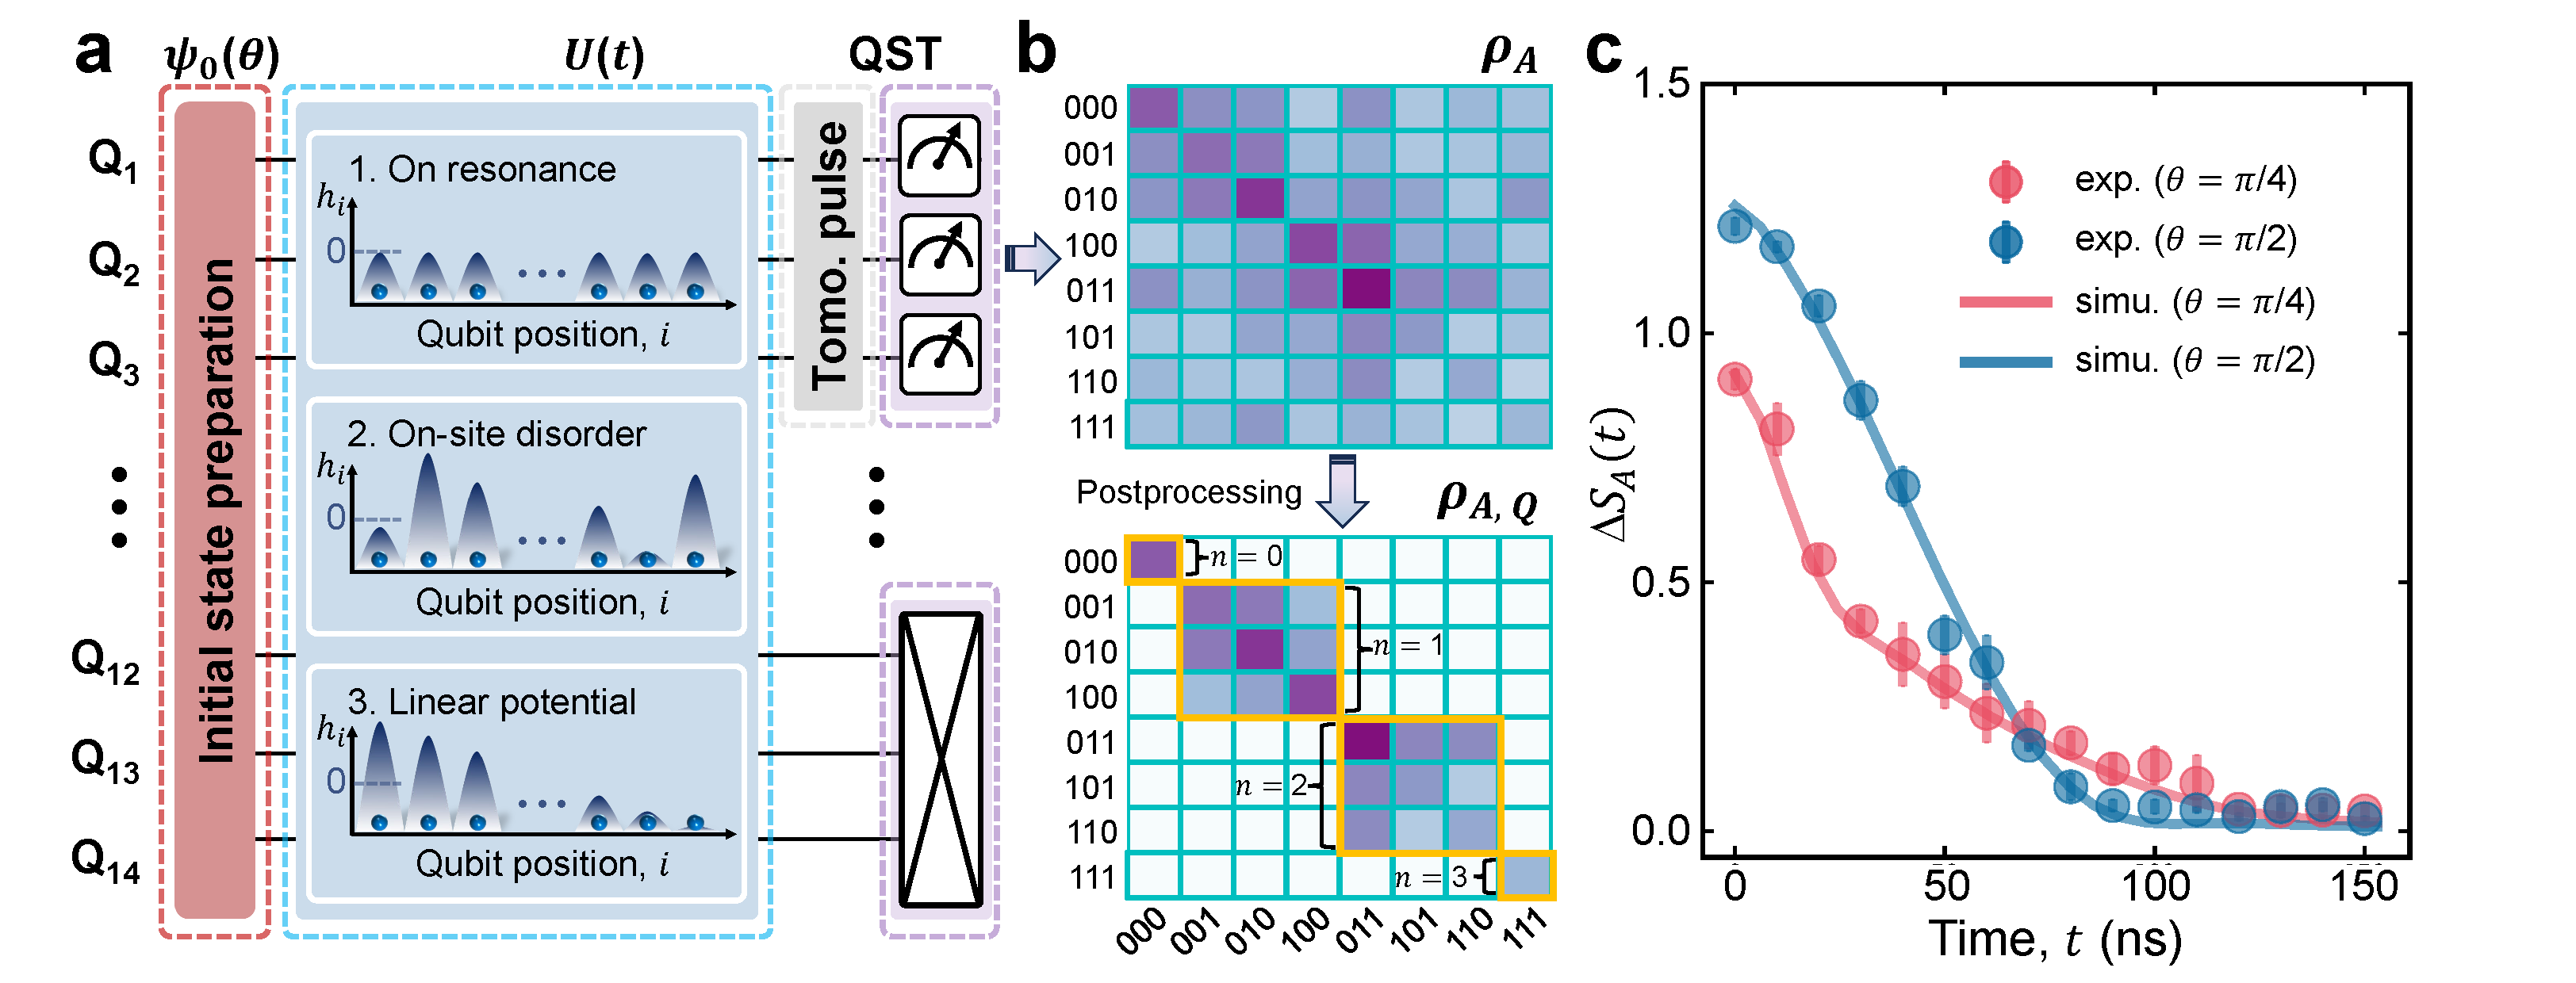
\includegraphics[width=0.95\textwidth]{Figure2/Figure2.pdf}
    \caption{
        \textcolor{blue}{强短程耦合区间($r\approx 10$)EA测量实验协议及其动力学。}
        (a) 实验协议的量子电路图。在初始态$|\Psi(\theta)\rangle$制备后,系统在工程化哈密顿量$H$下演化:$|\Psi(t)\rangle = U(t)|\Psi(\theta)\rangle = e^{-iHt}|\Psi(\theta)\rangle$,其中对量子比特施加了不同类型的在位势(共振、无序或线性梯度场)。
        (b) 通过量子态层析重建子系统$A$的密度矩阵。将密度矩阵投影到电荷算符$Q_A$的本征空间后,应用经典后处理来估计EA。
        (c) 强短程耦合区间($r\approx 10$)下量子比特共振时,倾斜Néel初始态(角度$\theta=\pi/4$和$\pi/2$)的EA动力学。观察到$\theta=\pi/2$时对称性恢复更快,并出现明显的交叉现象,证实了QME的存在。符号为实验数据,实线为包含退相干的理论结果。误差棒表示10次实验重复的标准偏差,每次包含3000次测量。
    }
    \label{fig:EA_measurement_strong_coupling}
\end{figure}



\textcolor{blue}{实验细节与关键发现:}
\begin{itemize}
    \item \textcolor{blue}{初始态制备:} 倾斜Néel态$|\theta\rangle_N = \bigotimes_{j=1}^{14} R_y(\theta)|s_j\rangle$,其中$|s_j\rangle = |0\rangle$($j$为奇数)或$|1\rangle$($j$为偶数)
    \item \textcolor{blue}{对称性破缺程度:} 倾斜角$\theta$控制全局$U(1)$对称性破缺程度:
    \begin{itemize}
        \item $\theta=0$或$\pi$:所有自旋沿$\sigma_z$方向排列(完全对称)
        \item $\theta=\pi/2$:所有自旋沿$\sigma_x$方向排列(最大对称性破缺)
    \end{itemize}
    \item \textcolor{blue}{耦合参数:} 
    \begin{itemize}
        \item 最近邻耦合:$g_N/2\pi = -5$ MHz
        \item 长程耦合:$g_L/2\pi \approx 0.5$ MHz
        \item 耦合比:$r \approx 10$
    \end{itemize}
    \item \textcolor{blue}{QME特征:} 虽然$|\theta=\pi/2\rangle_N$的初始EA高于$|\theta=\pi/4\rangle_N$,但其更快的对称性恢复导致更快的衰减率,产生明显的交叉现象
    \item \textcolor{blue}{物理机制:} 源于准粒子介导的弛豫,较大倾斜角$\theta$优先激发传播更快的模式,从而加速对称性恢复
\end{itemize}

\textcolor{blue}{纠缠不对称性定义:}
\begin{equation}
\Delta S_A(t) = S(\rho_{A,Q}(t)) - S(\rho_A(t))
\end{equation}
其中:
\begin{itemize}
    \item $\rho_A$:子系统$A$的约化密度矩阵
    \item $\rho_{A,Q} = \sum_q \Pi_q \rho_A \Pi_q$:在守恒荷$Q_A$本征空间上的投影
    \item $S(\rho)$:冯·诺依曼熵
\end{itemize}




\begin{enumerate}
    \item 数据集、评价指标、基线方法
    \item 主要实验表格或图(可插入图片)
\end{enumerate}

\begin{figure}[H]
    \centering
    % \includegraphics[width=0.6\textwidth]{figs/result.png}
    \caption{示例:结果对比图(替换为真实图片)}
\end{figure}

% ————— 优缺点与评价 —————
\section{优点与局限}
\begin{enumerate}
    \item 优点:列出 3-5 点
    \item 局限:理论/实践/资源/泛化等问题
    \item 可信度评估:是否做了消融、显著性检验、多个 seed 等
\end{enumerate}

% ————— 思路与扩展 —————
\section{灵感与后续方向}
\begin{enumerate}
    \item 可借鉴的技巧与工具
    \item 可尝试的改进点
    \item 与自己研究的结合点(短期/中期)
\end{enumerate}

% ————— 实现笔记 —————
\section{实现/复现笔记}
\begin{enumerate}
    \item 关键超参表
    \item 训练资源与耗时
    \item 遇到的问题与解决方案(环境、数据预处理、模型不收敛等)
\end{enumerate}

% ————— 复现检查表 —————
\section{复现检查表}
\begin{enumerate}
    \item [\(\square\)] 数据集下载与预处理
    \item [\(\square\)] 代码实现(模型/训练/评估)
    \item [\(\square\)] 与论文结果对齐
    \item [\(\square\)] 随机种子与多次实验
\end{enumerate}

% ————— 重要引用 —————
\section{参考与延伸阅读}
% 使用 BibTeX 时在同目录下放 refs.bib 并取消注释下面两行
% \bibliographystyle{apalike}
% \bibliography{refs}
列出文章引用或推荐的延伸阅读(手动列出或使用 BibTeX)。

% ————— 个人笔记与 TODO —————
\section{个人笔记 }
\textcolor{blue}{什么是本征?}
“本征”这个词源于德语“eigen”,意思是“自己的”、“固有的”、“特征的”。
\textcolor{red}{本征方程}是指一个线性算子作用在本征态上时,其结果等于\textcolor{red}{本征值}乘以\textcolor{red}{本征态}本身。形式上,设$\hat{A}$是一个线性算子,$| \psi \rangle$是$\hat{A}$的本征向量,$\lambda$是$\hat{A}$在$| \psi \rangle$上的本征值,则有:
\begin{equation}
\hat{A} | \psi \rangle = \lambda | \psi \rangle
\end{equation}

\textcolor{red}{物理意义:}
如果一个系统处于算符 $\hat{A}$ 的某个本征态上,那么你测量这个物理量 $\hat{A}$ 时,会得到一个确定无疑的结果,这个结果就是对应的本征值。

\vfill
{\small 记录时间:\today\ \currenttime}

\end{document}